\hypertarget{index_Introduction}{}\section{Introduction}\label{index_Introduction}
This library provides routines for running Reversible Jump Monte-\/\+Carlo Markov chains for data regression and forward models. See the \hyperlink{background}{Background} section for a general overview and references for more details.\hypertarget{index_How}{}\section{How to use}\label{index_How}
In order to find the right function to use, you need to know the following three things about your problem.


\begin{DoxyItemize}
\item What is the dimension of the problem?
\item Are the discontinuities in either value or gradient that you wish to determine/model?
\item Is your problem a regression problem or a forward model problem?
\end{DoxyItemize}

The diagram below and the following sections help explain how to classify your problem and the Directory below will help you identify which method to use for your problem and have a link to an example program using that method.

 
\begin{DoxyImageNoCaption}
  \mbox{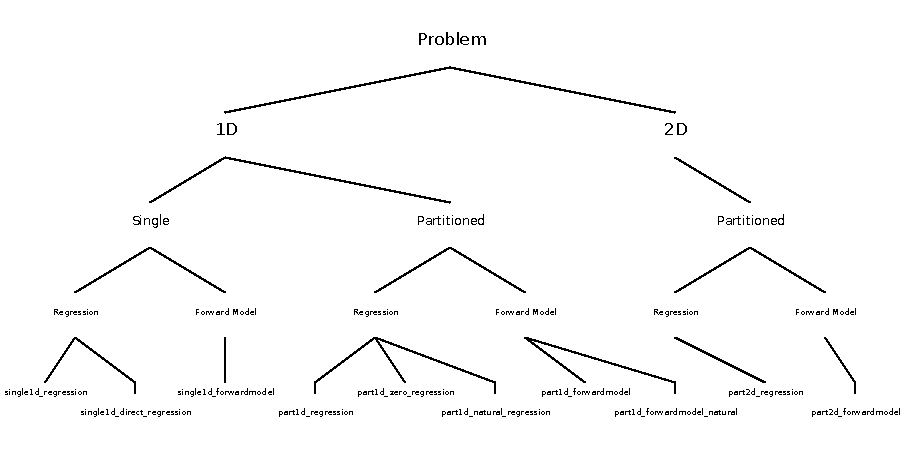
\includegraphics[width=\textwidth,height=\textheight/2,keepaspectratio=true]{main_tree}}
\end{DoxyImageNoCaption}
\hypertarget{index_Dimensionality}{}\subsection{Dimensionality}\label{index_Dimensionality}
The rjmcmc library supports 1 and 2 dimensional regression/forward model problems. If your problem consists of a regression/forward model of a single set of coordinates to a single set of values then it is a 1-\/dimensional problem. If your problem consists of a regression/forward model of a single set of coordinate pairs (eg x, y) to a single set of values then it is a 2-\/dimensional problem.\hypertarget{index_Partitioned}{}\subsection{Partitioned versus Single}\label{index_Partitioned}
If so you will want to use a partitioned or transdimensional approach, otherwise you can use the single methods (ie single partition methods).\hypertarget{index_Regression}{}\subsection{Regression versus Forward Model}\label{index_Regression}
A regression problem is one where there is a direct relationship between your data values and the fit to be generated. An example might be if your data consists of temperature measurements over time and you wanted to generate the temperature over time curve, then this is a regression problem. If instead you had a profile of the temperature down a bore and wanted to reconstruct the temperature versus time at the surface of the bore then this is a forward model problem. With forward model problems you will need to provide your own code for the forward model and calculate the log of the likelihood. In the case the borehole example, the rjmcmc library will provide a trial surface temperature record and the forward model will consist of a integration of the heat-\/diffusion equation given this input to create a trial borehole temperature profile. The likelihood is then calculated from the sum of the squared errors between the measured and trial borehole temperature profiles.\hypertarget{index_Directory}{}\section{Directory}\label{index_Directory}
\hypertarget{index_singleregress1d}{}\subsection{1\+D Single Partition Regression}\label{index_singleregress1d}
The following functions are available\+:


\begin{DoxyItemize}
\item \hyperlink{regression_8h_a037d789bc3de5c4c55b0c781193ae3b7}{single1d\+\_\+regression} uses an automatic prior to determine the best weights to be given to the order of the fitting polynomial.
\item \hyperlink{regression_8h_ac8c2d9357e8a0ac1ff03fc48843e804b}{single1d\+\_\+regression\+\_\+with\+\_\+prior} uses a user supplied prior to sample varying order polynomials to fit the data (deprecated/used for testing).
\item \hyperlink{regression_8h_a0ab9525ab0dc478cfa18bc9bd5a94d97}{single1d\+\_\+direct\+\_\+regression} use direct integration to determine the best fit to the data (deprecated/used for testing).
\end{DoxyItemize}

The following example codes are available (available under the Examples tab)\+:


\begin{DoxyItemize}
\item 1d/single/regression/cubic/cubic.\+c performs a regression on a known cubic function with added gaussian noise.
\end{DoxyItemize}\hypertarget{index_partregress1d}{}\subsection{1\+D Partitioned Regression}\label{index_partregress1d}
The following functions are available\+:


\begin{DoxyItemize}
\item \hyperlink{regression_8h_a17bc74fa9fb9c6287ab4e19751c6bb17}{part1d\+\_\+regression} uses an automatic prior to determine the best weights for the polynomial order(s) within each partition.
\item \hyperlink{regression_8h_ab17dfbf7aa5a8f0ba54441e7e9dc33cf}{part1d\+\_\+zero\+\_\+regression} use 0th order polynomials within each partition.
\item \hyperlink{regression_8h_abd2a0dc74a4bb3934c21c7864759bbbd}{part1d\+\_\+natural\+\_\+regression} use connected line segments between each partition boundary to provide a continuous fit (with change points becoming changes in gradients).
\end{DoxyItemize}

The following example codes are available (available under the Examples tab)\+:


\begin{DoxyItemize}
\item 1d/partitioned/regression/multiquad/multiquad.\+c performs a regression on a function comprised of piece wise quadratic functions with discontinuties with added gaussian noise.
\item 1d/partitioned/regression/multistep/multistep.\+c
\item 1d/partitioned/regression/sawtooth/sawtooth.\+c
\item 1d/partitioned/regression/zeromultistep/zeromultistep.\+c
\end{DoxyItemize}\hypertarget{index_singlefm1d}{}\subsection{1\+D Single Partition Forward Model}\label{index_singlefm1d}
The following functions are available\+:


\begin{DoxyItemize}
\item \hyperlink{forwardmodel_8h_a65b1200fd2ef808c85b1915fa1413b58}{single\+\_\+forwardmodel} performs a forward model analysis on an arbitrary number of parameters.
\item \hyperlink{forwardmodel__f_8h_a11799898f79291bad341135f00b7a243}{single\+\_\+forwardmodel\+\_\+f} is a fortran 2003 interface to the \hyperlink{forwardmodel_8h_a65b1200fd2ef808c85b1915fa1413b58}{single\+\_\+forwardmodel} function.
\item \hyperlink{forwardmodel_8h_a95b892df15e3e7b58497a68af64a7b0d}{single\+\_\+forwardmodel\+\_\+hierarchical} performs a forward model analysis on an arbitrary number of parameters with a custom hierarchical peturbation of the covariance matrix.
\end{DoxyItemize}

The following example codes are available (available under the Examples tab)\+:


\begin{DoxyItemize}
\item 1d/single/fm/simplef/simplef.\+f90
\item 1d/single/fm/simpleimage/simpleimage.\+c
\item 1d/single/fm/spherefit/spherefit.\+c
\end{DoxyItemize}\hypertarget{index_partfm1d}{}\subsection{1\+D Partitioned Forward Model}\label{index_partfm1d}
The following functions are available\+:


\begin{DoxyItemize}
\item \hyperlink{forwardmodel_8h_a852beb6cfb6875927200fa90d6d60d6e}{part1d\+\_\+forwardmodel}
\item \hyperlink{forwardmodel__f_8h_aa7d79eacccaac4d0770cd207b166dced}{part1d\+\_\+forwardmodel\+\_\+f}
\item \hyperlink{forwardmodel_8h_a267826c400d1ae8be3473c4bdc03e05b}{part1d\+\_\+forwardmodel\+\_\+hierarchical}
\item \hyperlink{forwardmodel_8h_a736c12ab94ec4dd7e785baa8b028c6e6}{part1d\+\_\+forwardmodel\+\_\+natural}
\item \hyperlink{forwardmodel_8h_ad6b46c9104fbbea5c119bc64e8f29190}{part1d\+\_\+forwardmodel\+\_\+natural\+\_\+hierarchical}
\end{DoxyItemize}

The following example codes are available (available under the Examples tab)\+:


\begin{DoxyItemize}
\item 1d/partitioned/fm/functionfit/functionfit.\+c
\item 1d/partitioned/fm/functionfitf/functionfitf.\+f90
\item 1d/partitioned/fm/regression/regression.\+c
\end{DoxyItemize}\hypertarget{index_partregress2d}{}\subsection{2\+D Partitioned Regression}\label{index_partregress2d}
The following functions are available\+:


\begin{DoxyItemize}
\item \hyperlink{regression_8h_aa4589a0fbb1ca56b2db6fafbda40161f}{part2d\+\_\+regression}
\end{DoxyItemize}\hypertarget{index_partfm2d}{}\subsection{2\+D Partitioned Forward Model}\label{index_partfm2d}
The following functions are available\+:


\begin{DoxyItemize}
\item \hyperlink{forwardmodel_8h_a1a30e27827e21f0906d74634c611cc54}{part2d\+\_\+forwardmodel}
\item \hyperlink{forwardmodel_8h_a7f812853c942aeb44dd57ce2823a8523}{part2d\+\_\+forwardmodel\+\_\+hierarchical} 
\end{DoxyItemize}